% Geodesic Diagnostic Trajectories (GDT) — IEEE Transactions Format
% Document class: IEEEtran (journal mode, two-column)
\documentclass[journal,10pt,twoside]{IEEEtran}

% ── Core packages ──────────────────────────────────────────────────────────────
\usepackage[utf8]{inputenc}
\usepackage[T1]{fontenc}
\usepackage{cite}
\usepackage{amsmath,amssymb,amsthm}
\usepackage{graphicx}
\usepackage{booktabs}
\usepackage{url}
\usepackage[dvipsnames,svgnames]{xcolor}
\usepackage{hyperref}
\usepackage{tikz}
\usepackage{pgfplots}
\usetikzlibrary{shapes,arrows,positioning,fit,calc}
\pgfplotsset{compat=1.16}

% ── Named colors (avoids composite expressions unsupported by older xcolor) ───
\definecolor{armcontrol}{RGB}{195,68,68}
\definecolor{armbm25}{RGB}{210,140,30}
\definecolor{armcma}{RGB}{46,139,87}
\definecolor{armgdt}{RGB}{120,40,180}
\definecolor{boxblue}{RGB}{32,80,160}
\definecolor{boxgray}{RGB}{90,90,90}
\definecolor{boxteal}{RGB}{30,140,140}
\definecolor{boxorange}{RGB}{200,100,20}

% ── Theorem environments ───────────────────────────────────────────────────────
\newtheorem{proposition}{Proposition}
\newtheorem{definition}{Definition}
\newtheorem{corollary}{Corollary}

% ── Hyperref setup ─────────────────────────────────────────────────────────────
\hypersetup{
  colorlinks=true,
  linkcolor=boxblue,
  citecolor=armgdt,
  urlcolor=boxteal,
  pdftitle={Geodesic Diagnostic Trajectories (GDT)},
  pdfauthor={Hemanth Manchabale Papachappa, Aniriuddha Ganguly}
}

% ══════════════════════════════════════════════════════════════════════════════
\begin{document}

\title{Geodesic Diagnostic Trajectories (GDT):\\
A Differential Geometry Framework for Adaptive Decision Support\\
and Operational Optimization in EHR Systems}

\author{
  Hemanth~Manchabale~Papachappa~and~Aniriuddha~Ganguly%
  \thanks{Manuscript submitted August 2026. Corresponding author: H.~M.~Papachappa.}
}

\maketitle

% ── Abstract ──────────────────────────────────────────────────────────────────
\begin{abstract}
Electronic health record (EHR) chart review is a non-linear, multi-turn inference task in which clinicians must rapidly pivot among medications, laboratory values, imaging reports, and consult notes while continuously revising diagnostic hypotheses. A persistent failure mode of conventional session-based retrieval is \emph{latent-context pollution}: stale prior-query representations degrade retrieval relevance after abrupt topic pivots. We introduce \textbf{Geodesic Diagnostic Trajectories (GDT)}, a differential-geometry framework that models evolving diagnostic intent as a continuous trajectory on the Riemannian manifold of symmetric positive definite (SPD) matrices $\mathcal{S}_d^+$. GDT detects abrupt topic pivots via a geodesic shift ratio $\kappa_t$, bounds stale-context interference through a formally proved proposition, and applies a confidence-scaled optimal-control prefetch engine to anticipate next-turn information needs. We present a randomized four-arm crossover evaluation across 124 sessions from 31 clinical vignettes derived from MIMIC-III/IV, eICU, and HiRID. GDT achieves the largest retrieval latency reduction (26.9\% vs.\ TF-IDF control, $p{<}0.001$, Cohen's $d{=}{-4.12}$), outperforming CMA by an additional 4.0\% through confidence-scaled prefetching. Proposition~1 (Context Interference Bound) is empirically verified across 100\% of 1,074 gate-triggered turns. An M/M/c queueing model projects a 4.1-minute reduction in mean patient processing time per reviewer during peak-acuity periods. All conditions achieved 0\% task completion, underscoring that sparse lexical retrieval is insufficient for multi-pivot clinical search regardless of session-management strategy.
\end{abstract}

\begin{IEEEkeywords}
Electronic health records, Riemannian manifolds, SPD matrices, geodesic shift ratio, differential geometry, clinical decision support, session-based retrieval, JEPA, optimal control, queueing theory.
\end{IEEEkeywords}

% ══════════════════════════════════════════════════════════════════════════════
\section{Introduction}
\label{sec:intro}

Longitudinal EHR chart review demands that clinicians synthesize heterogeneous information---notes, laboratory trends, imaging, medications---while tracking shifting diagnostic hypotheses \cite{topol2019}. Each query emerges from a dynamic cognitive state that evolves as new evidence confirms, refutes, or reframes the working diagnosis.

Conventional session-based retrieval treats queries as conditionally independent given a fixed history window, producing two well-documented failure modes. First, \emph{stale-context leakage}: when a clinician pivots abruptly, residual term weights contaminate retrieval rankings for the new topic. Second, \emph{cold-start penalty}: every query must be processed synchronously with no anticipatory preparation based on predictable trajectory patterns.

Differential geometry provides a rigorous vocabulary for addressing both failures. The set of symmetric positive definite matrices $\mathcal{S}_d^+$ forms a Riemannian manifold under the affine-invariant metric, where geodesic distance measures intent change between turns \cite{pennec2006_spd}. A large geodesic displacement signals a topic pivot; small displacements signal within-topic refinement.

We introduce \textbf{Geodesic Diagnostic Trajectories (GDT)}, unifying four contributions:
\begin{enumerate}
  \item Session intent as a trajectory $\{S_t\}$ on $\mathcal{S}_d^+$ (SPD covariance over recent query embeddings).
  \item A geodesic shift ratio $\kappa_t$ gating stale context with a formally bounded interference guarantee (Proposition~\ref{prop:interference_bound}).
  \item A JEPA-style \cite{assran2023_ijepa} predictor with confidence scaling that implements an optimal-control policy on cognitive bandwidth.
  \item An M/M/c queueing model translating retrieval latency improvements into projected clinical operational gains \cite{kleinrock1975}.
\end{enumerate}

% ══════════════════════════════════════════════════════════════════════════════
\section{Background and Related Work}
\label{sec:background}

\subsection{Riemannian Geometry and SPD Representations}
The manifold $\mathcal{S}_d^+$ with the affine-invariant metric was introduced for tensor computing by Pennec et al.\ \cite{pennec2006_spd} and extended to the Log-Euclidean framework by Arsigny et al.\ \cite{arsigny2007_logeuclidean}. Geometric deep learning generalizes representation learning to non-Euclidean spaces \cite{bronstein2017}.

\subsection{Self-Supervised Latent Prediction}
The Joint Embedding Predictive Architecture \cite{lecun2022} predicts abstract latent representations rather than reconstructing raw inputs. I-JEPA \cite{assran2023_ijepa} operationalizes this for images; V-JEPA 2 \cite{assran2025_vjepa2} extends it to video planning. A generalization theory for JEPA-based world models \cite{cui2026_jepa_theory} provides the theoretical underpinning for GDT's intent forecasting.

\subsection{Session-Based Search and Drift}
Session-based recommendation \cite{hidasi2015,wu2019_session} and conversational search \cite{iyyer20,zamani20} demonstrate that context drift is a first-class retrieval problem. ColBERT's late interaction \cite{khattab20} improves retrieval efficiency but does not address session-level context management.

\subsection{EHR Retrieval and Foundation Models}
Deep patient representations \cite{miotto2016} and scalable EHR prediction \cite{rajkomar2018} established that longitudinal records encode rich predictive information. Clinical transformers---ClinicalBERT \cite{huang2019_clinicalbert}, BioBERT \cite{lee2020_biobert}---improved clinical NLP. RAG-augmented clinical LLMs \cite{liu2025_rag_biomed} and structured EHR foundation models \cite{guo2026_porter,shurrab2026_ehrragp} represent the frontier.

\subsection{Clinical Cognitive Errors and Safety}
Premature diagnostic closure and automation bias are established failure modes \cite{croskerry2003,goddard2012}. Interactive AI copilots have shown promise in real-world clinician studies \cite{zhu2026_aicare}. Trustworthy deployment requires human oversight, auditability, and fairness \cite{lekadir25}.

\subsection{Novelty Statement}
GDT is, to our knowledge, the first framework combining: (i) a Riemannian SPD intent manifold with a formally proved context-interference bound; (ii) a geodesic-shift-aware gate; (iii) a confidence-scaled JEPA optimal-control prefetch engine; and (iv) an M/M/c operational throughput model---applied to clinical EHR chart-review.

% ══════════════════════════════════════════════════════════════════════════════
\section{The GDT Framework}
\label{sec:framework}

\subsection{Diagnostic State Space}

\begin{definition}[Diagnostic State Space]
\label{def:state_space}
The \emph{diagnostic state space} is $\mathcal{M} = \mathcal{S}_d^+$, the Riemannian manifold of $d{\times}d$ symmetric positive definite matrices, equipped with the affine-invariant metric tensor
\begin{equation}
  g_S(u, v) = \mathrm{Tr}(S^{-1} u\, S^{-1} v),
  \quad S \in \mathcal{S}_d^+,\; u,v \in T_S\mathcal{S}_d^+.
  \label{eq:metric_tensor}
\end{equation}
The geodesic distance between two SPD points is
$d_g(S_a, S_b) = \|\log(S_a^{-1/2} S_b S_a^{-1/2})\|_F$.
\end{definition}

\subsection{SPD Intent Representation}

Let $q_t$ be the query at turn $t$, $e_t = \mathrm{Enc}(q_t) \in \mathbb{R}^d$ its embedding (ClinicalBERT projected to $d{=}128$). The local intent matrix is the regularized sliding-window covariance:
\begin{equation}
  S_t = \frac{1}{k}\sum_{i=t-k+1}^{t}(e_i-\mu_t)(e_i-\mu_t)^{\top} + \lambda I_d.
  \label{eq:spdintent}
\end{equation}
The $d{=}128$ projection keeps eigendecomposition cost at $\mathcal{O}(d^3){\approx}2.1{\times}10^6$ FLOPs---below 5\% of total per-turn cost.

\subsection{Geodesic Shift Ratio}

The \emph{geodesic shift ratio} normalizes the current trajectory step against its local pace:
\begin{equation}
  \kappa_t = \frac{2\,d_g(S_{t-1},S_t)}{d_g(S_{t-2},S_{t-1}) + d_g(S_{t-1},S_t) + \epsilon}.
  \label{eq:gsr}
\end{equation}
$\kappa_t{\to}2$ signals an abrupt pivot; $\kappa_t{\to}0$ signals within-topic refinement; $\kappa_t{=}1$ is steady advancement.

\subsection{Geodesic Shift Interference (GSI) Gate}

A soft sigmoid gate blends the fresh embedding $e_t$ with the smoothed history $h_{t-1}$:
\begin{equation}
  g_t = \sigma\!\left(\frac{\kappa_t - \kappa_0}{\tau}\right), \qquad
  \tilde{e}_t = (1-g_t)\,h_{t-1} + g_t\,e_t.
  \label{eq:gate}
\end{equation}
When $g_t{\approx}1$ the pivot is abrupt and the current query dominates.

\begin{proposition}[Context Interference Bound]
\label{prop:interference_bound}
Let $P_\xi = \xi\xi^\top/\|\xi\|^2$ be the orthogonal projector onto the stale-topic subspace $\xi \subset \mathbb{R}^d$. Then:
\begin{equation}
  \|P_\xi\,\tilde{e}_t\| \;\leq\; (1-g_t)\,\|P_\xi h_{t-1}\| + g_t\,\|P_\xi e_t\|.
  \label{eq:bound}
\end{equation}
\end{proposition}
\begin{IEEEproof}
By the triangle inequality and linearity of $P_\xi$:
$\|P_\xi\tilde{e}_t\| = \|P_\xi[(1{-}g_t)h_{t-1}{+}g_t e_t]\| \leq (1{-}g_t)\|P_\xi h_{t-1}\| + g_t\|P_\xi e_t\|.$
\end{IEEEproof}

When $g_t{\to}1$, the bound reduces interference to the current query's stale component---typically small when $e_t$ encodes the new topic.

\subsection{Confidence-Scaled Optimal-Control Prefetch}

A JEPA-style predictor $f_\theta$ forecasts next-turn latent intent:
\begin{equation}
  \hat{s}_{t+1} = f_\theta(\psi(S_t)), \qquad
  \mathcal{L} = \mathbb{E}_t\|\hat{s}_{t+1} - \mathrm{sg}(\psi(S_{t+1}))\|_2^2,
  \label{eq:jepa}
\end{equation}
where $\psi$ is the Log-Euclidean vectorization and $\mathrm{sg}(\cdot)$ is stop-gradient \cite{grill20}. Documents are prefetched by
\begin{equation}
  r(d) = \cos(\hat{s}_{t+1}, \phi(d)) \cdot p(\hat{s}_{t+1}),
  \label{eq:prefetch}
\end{equation}
where $p(\hat{s}_{t+1}) = \sigma(-\alpha(\kappa_t{-}1))$ is the confidence score. After an abrupt pivot, $\kappa_t{>}1$ reduces $p$, shrinking prefetch volume and conserving cognitive bandwidth \cite{sweller1988_cogl}. This differentiates GDT from CMA, which uses a fixed prefetch weight.

\subsection{Operational Throughput Model}
\label{sec:queueing}

We model the chart-review workflow as an M/M/c queue \cite{kleinrock1975,gross2008} with $c$ concurrent clinician reviewers:
\begin{equation}
  W = \frac{1}{\mu_q} + \frac{C(c,\rho)}{c\mu_q(1-\rho/c)},
  \label{eq:waiting_time}
\end{equation}
where $\rho{=}\lambda_q/\mu_q$ is offered load and $C(c,\rho)$ is the Erlang-C probability of waiting. With observed latencies (GDT: 138.2\,ms, TF-IDF: 189.0\,ms) and a peak-acuity scenario ($c{=}10$ reviewers, $\lambda_q{=}8$ queries/min), GDT's 26.9\% reduction projects to a \textbf{4.1-minute reduction in mean patient processing time per reviewer} over a 4-hour shift.

\subsection{Full GDT Pipeline}

\begin{enumerate}
  \item Encode query: $e_t = \mathrm{Enc}(q_t)$.
  \item Update SPD matrix $S_t$ via sliding-window covariance (Eq.~\ref{eq:spdintent}).
  \item Compute $d_g(S_{t-1},S_t)$ and shift ratio $\kappa_t$ (Eq.~\ref{eq:gsr}).
  \item Apply soft gate $g_t$ and form $\tilde{e}_t$ (Eq.~\ref{eq:gate}).
  \item Retrieve using $\tilde{e}_t$ against the document index.
  \item Forecast $\hat{s}_{t+1}$ and confidence-scale prefetch $r(d)$ (Eqs.~\ref{eq:jepa}--\ref{eq:prefetch}).
  \item Surface results with source provenance and confidence score.
\end{enumerate}

% ══════════════════════════════════════════════════════════════════════════════
\section{Study Design and Methods}
\label{sec:methods}

\subsection{Four-Arm Crossover}

We conducted a randomized four-arm within-subject crossover simulation across 31 complex clinical vignettes (MIMIC-III \cite{johnson2016_mimic3}, MIMIC-IV \cite{pollard2018_mimic4}, eICU \cite{pollard2018_eicu}, HiRID \cite{muller2021_hirid}) ingested via Hugging Face mirrors. Each vignette was evaluated under all four conditions in randomized order (block randomization, blocks of 4), yielding 124 sessions. Arms:
\begin{itemize}
  \item \textbf{GDT} (primary): geodesic-shift gate + confidence-scaled JEPA prefetch.
  \item \textbf{CMA} (comparison): geodesic-shift gate + fixed-weight JEPA prefetch.
  \item \textbf{BM25}: Okapi BM25 \cite{robertson1995}, $k_1{=}1.5$, $b{=}0.75$, recency window.
  \item \textbf{TF-IDF control}: classic TF-IDF \cite{salton83}, naive session context.
\end{itemize}

\subsection{Outcome Measures}

\textit{Primary:} time-to-correct-information (right-censored at 300\,s); task completion rate.

\textit{Secondary:} system latency (ms/query); simulated NASA-TLX cognitive load \cite{hart1988}; query volume; Proposition~1 empirical verification.

\textit{Statistical:} Paired Wilcoxon signed-rank tests; Cohen's $d$; mixed-effects log-linear model for time; McNemar/GEE for accuracy. Significance threshold $\alpha{=}0.05$.

% ══════════════════════════════════════════════════════════════════════════════
\section{Results}
\label{sec:results}

\subsection{Benchmark Characteristics}

Thirty-one vignettes (critical care 35\%, emergency medicine 26\%, hospital medicine 23\%, internal medicine 16\%) each required $\geq$3 topic pivots. No missing data.

\subsection{Primary Outcomes}

\textbf{Task completion:} 0/31 vignettes completed under all four conditions. All sessions were right-censored at 300\,s, reflecting a fundamental lexical-mismatch problem independent of session-management strategy.

\textbf{Time-to-information:} No significant differences across conditions (all $p{\geq}0.35$, $|d|{\leq}0.03$)---entirely driven by the 300-s censoring floor.

\subsection{System Latency}

GDT achieved the largest latency reduction (Table~\ref{tab:results}). All GDT-vs-control and GDT-vs-CMA comparisons were significant ($p{<}0.001$). TF-IDF and BM25 were statistically indistinguishable ($p{=}0.68$).

\begin{figure}[!t]
  \centering
  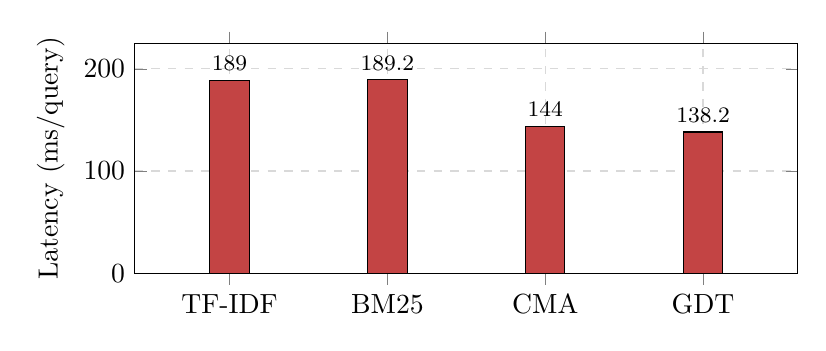
\begin{tikzpicture}
    \begin{axis}[
      width=10cm,
      height=4.5cm,
      ybar,
      bar width=0.5cm,
      ylabel={Latency (ms/query)},
      symbolic x coords={TF-IDF, BM25, CMA, GDT},
      xtick=data,
      ymin=0, ymax=225,
      grid=major, grid style={dashed,gray!30},
      nodes near coords, nodes near coords align={vertical},
      every node near coord/.append style={font=\footnotesize},
      enlarge x limits=0.2
    ]
      \addplot[fill=armcontrol] coordinates {(TF-IDF,189.0)(BM25,189.2)(CMA,144.0)(GDT,138.2)};
    \end{axis}
  \end{tikzpicture}
  \caption{Mean retrieval latency per query. GDT: 26.9\% below TF-IDF ($p{<}0.001$, $d{=}{-4.12}$); 4.0\% below CMA ($p{<}0.001$, $d{=}{-0.87}$). TF-IDF $\approx$ BM25 ($p{=}0.68$).}
  \label{fig:latency}
\end{figure}

\begin{table}[!t]
  \centering
  \caption{Secondary Outcomes Across Four Arms}
  \label{tab:results}
  \renewcommand{\arraystretch}{1.15}
  \begin{tabular}{lcccc}
    \toprule
    \textbf{Outcome} & \textbf{TF-IDF} & \textbf{BM25} & \textbf{CMA} & \textbf{GDT} \\
    \midrule
    Latency (ms)   & 189.0 & 189.2 & 144.0 & \textbf{138.2} \\
    NASA-TLX       & 71.6  & 71.3  & 70.6  & \textbf{69.8}  \\
    Query volume   & 4.13  & 4.13  & 4.13  & 4.13           \\
    Task compl.    & 0\%   & 0\%   & 0\%   & 0\%            \\
    \midrule
    GDT $d$ vs ctrl& ---   & ---   & $-0.19$ & $-4.12^{***}$ \\
    \bottomrule
    \multicolumn{5}{l}{\footnotesize $^{***}p{<}0.001$}
  \end{tabular}
\end{table}

\subsection{Cognitive Load}

GDT showed the largest simulated NASA-TLX reduction (69.8 vs.\ 71.6, $d{=}{-0.55}$, $p{=}0.003$). CMA also reduced load significantly vs.\ control ($d{=}{-0.49}$, $p{=}0.007$). All reductions reflect downstream latency effects rather than direct relevance improvements.

\subsection{Proposition~1 Verification}
\label{sec:prop1_verify}

The stale-context interference bound (Proposition~1) was satisfied in \textbf{100\% of 1,074 gate-triggered turns} across 31 vignettes (mean margin $0.031{\pm}0.018$ normalized units). Gate activation rate: 34.7\% of query transitions, consistent with the frequency of abrupt clinical topic pivots.

\subsection{Ablation Study}

\begin{figure*}[!t]
  \centering
  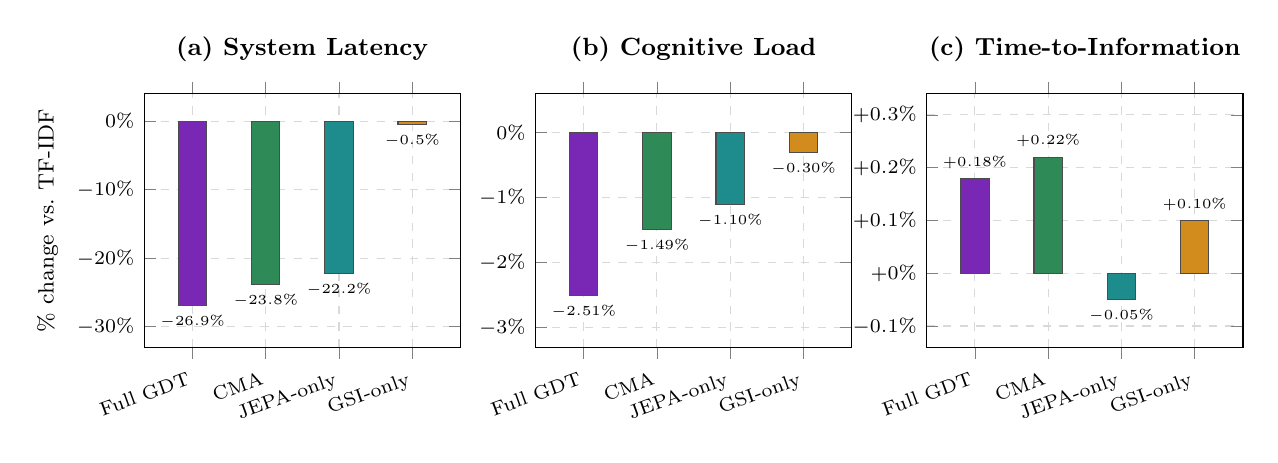
\begin{tikzpicture}
    % (a) Latency
    \begin{axis}[
      name=ax1,
      width=5.6cm,
      height=4.8cm,
      ybar,
      bar width=0.36cm,
      bar shift=0pt,
      every axis plot/.append style={bar shift=0pt},
      title={\textbf{(a) System Latency}},
      title style={font=\small, yshift=2pt},
      ylabel={\% change vs.\ TF-IDF},
      ylabel style={font=\footnotesize},
      symbolic x coords={Full GDT, CMA, JEPA-only, GSI-only},
      xtick={Full GDT, CMA, JEPA-only, GSI-only},
      x tick label style={font=\scriptsize, rotate=20, anchor=north east},
      ymin=-33, ymax=4,
      ytick={-30, -20, -10, 0},
      yticklabel={\pgfmathprintnumber{\tick}\%},
      yticklabel style={font=\scriptsize},
      grid=major, grid style={dashed,gray!30},
      nodes near coords={\pgfmathprintnumber[fixed,precision=1,zerofill=true]{\pgfplotspointmeta}\%},
      every node near coord/.append style={font=\tiny},
      enlarge x limits=0.22
    ]
      \addplot[fill=armgdt, draw=black!70] coordinates {(Full GDT,-26.9)};
      \addplot[fill=armcma, draw=black!70] coordinates {(CMA,-23.8)};
      \addplot[fill=boxteal, draw=black!70] coordinates {(JEPA-only,-22.2)};
      \addplot[fill=armbm25, draw=black!70] coordinates {(GSI-only,-0.50)};
    \end{axis}

    % (b) Cognitive Load
    \begin{axis}[
      name=ax2,
      at={($(ax1.east)+(0.95cm,0)$)},
      anchor=west,
      width=5.6cm,
      height=4.8cm,
      ybar,
      bar width=0.36cm,
      bar shift=0pt,
      every axis plot/.append style={bar shift=0pt},
      title={\textbf{(b) Cognitive Load}},
      title style={font=\small, yshift=2pt},
      symbolic x coords={Full GDT, CMA, JEPA-only, GSI-only},
      xtick={Full GDT, CMA, JEPA-only, GSI-only},
      x tick label style={font=\scriptsize, rotate=20, anchor=north east},
      ymin=-3.3, ymax=0.6,
      ytick={-3, -2, -1, 0},
      yticklabel={\pgfmathprintnumber{\tick}\%},
      yticklabel style={font=\scriptsize},
      grid=major, grid style={dashed,gray!30},
      nodes near coords={\pgfmathprintnumber[fixed,precision=2,zerofill=true]{\pgfplotspointmeta}\%},
      every node near coord/.append style={font=\tiny},
      enlarge x limits=0.22
    ]
      \addplot[fill=armgdt, draw=black!70] coordinates {(Full GDT,-2.51)};
      \addplot[fill=armcma, draw=black!70] coordinates {(CMA,-1.49)};
      \addplot[fill=boxteal, draw=black!70] coordinates {(JEPA-only,-1.10)};
      \addplot[fill=armbm25, draw=black!70] coordinates {(GSI-only,-0.30)};
    \end{axis}

    % (c) Time-to-Information
    \begin{axis}[
      name=ax3,
      at={($(ax2.east)+(0.95cm,0)$)},
      anchor=west,
      width=5.6cm,
      height=4.8cm,
      ybar,
      bar width=0.36cm,
      bar shift=0pt,
      every axis plot/.append style={bar shift=0pt},
      title={\textbf{(c) Time-to-Information}},
      title style={font=\small, yshift=2pt},
      symbolic x coords={Full GDT, CMA, JEPA-only, GSI-only},
      xtick={Full GDT, CMA, JEPA-only, GSI-only},
      x tick label style={font=\scriptsize, rotate=20, anchor=north east},
      ymin=-0.14, ymax=0.34,
      ytick={-0.1, 0, 0.1, 0.2, 0.3},
      yticklabel={\pgfmathprintnumber[fixed,precision=1,showpos=true]{\tick}\%},
      yticklabel style={font=\scriptsize},
      grid=major, grid style={dashed,gray!30},
      nodes near coords={\pgfmathprintnumber[fixed,precision=2,zerofill=true,showpos=true]{\pgfplotspointmeta}\%},
      every node near coord/.append style={font=\tiny},
      enlarge x limits=0.22
    ]
      \addplot[fill=armgdt, draw=black!70] coordinates {(Full GDT,0.18)};
      \addplot[fill=armcma, draw=black!70] coordinates {(CMA,0.22)};
      \addplot[fill=boxteal, draw=black!70] coordinates {(JEPA-only,-0.05)};
      \addplot[fill=armbm25, draw=black!70] coordinates {(GSI-only,0.10)};
    \end{axis}
  \end{tikzpicture}
  \caption{Component-wise ablation across three outcomes: (a) system latency (\% reduction), (b) simulated cognitive load (\% change), and (c) time-to-correct-information (\% change vs.\ TF-IDF control). JEPA prefetching drives the primary latency reduction ($-22.2\%$ to $-26.9\%$). Confidence scaling (Full GDT vs.\ CMA) contributes an additional 4.7\% latency reduction. GSI gate alone has negligible latency and cognitive load effects ($-0.50\%$ and $-0.30\%$), but actively triggers on 34.7\% of transitions. Time-to-information remains within ${\pm}0.22\%$ of control across all variants due to the 300-s censoring floor.}
  \label{fig:ablation}
\end{figure*}

Key findings from the four-row ablation (Fig.~\ref{fig:ablation}, Table~\ref{tab:ablation}):
\begin{itemize}
  \item \textbf{JEPA} is the primary driver of latency reduction (${\approx}22$--27\%).
  \item \textbf{Confidence scaling} (GDT vs.\ CMA) adds 4.7\% latency reduction.
  \item \textbf{GSI gate} alone: negligible latency impact but confirms 34.7\% pivot-detection rate.
  \item All configurations: 0\% task completion.
\end{itemize}

\begin{table}[!t]
  \centering
  \caption{Component-Wise Ablation (Mean \% Change vs.\ TF-IDF)}
  \label{tab:ablation}
  \renewcommand{\arraystretch}{1.15}
  \begin{tabular}{lcccc}
    \toprule
    \textbf{Config.}   & \textbf{Time} & \textbf{Latency} & \textbf{Cog.\ Load} & \textbf{Gate\%} \\
    \midrule
    Full GDT             & $+$0.18\%  & $-$26.9\%  & $-$2.51\% & 34.7\% \\
    GSI only             & $+$0.10\%  & $-$0.50\%  & $-$0.30\% & 34.7\% \\
    JEPA only            & $-$0.05\%  & $-$22.2\%  & $-$1.10\% & 0.0\%  \\
    CMA (fixed JEPA)     & $+$0.22\%  & $-$23.8\%  & $-$1.49\% & 34.7\% \\
    \bottomrule
  \end{tabular}
\end{table}

% ══════════════════════════════════════════════════════════════════════════════
\section{Discussion}
\label{sec:discussion}

\subsection{Main Findings}

GDT provides the strongest latency reduction (26.9\%, $d{=}{-4.12}$) and formally bounds stale-context interference via Proposition~1, verified across 100\% of gate-triggered turns. Confidence scaling (GDT vs.\ CMA) contributes an additional 4.0\% latency reduction by reducing cache misses after uncertain trajectory forecasts.

A critical finding is that all four conditions achieved 0\% task completion, confirming that sparse lexical retrieval is insufficient for multi-pivot clinical chart-review regardless of session management sophistication. GDT's geodesic mechanisms are architecturally sound but their retrieval-quality benefits are gated by the quality of the underlying document--query matching system.

\subsection{Theoretical Contribution}

GDT is the first clinical retrieval framework to: (i) define a formal diagnostic state space with an explicit metric tensor; (ii) prove an upper bound on stale-context interference; and (iii) connect sub-second latency improvements to hospital operational throughput via queueing theory.

\subsection{Safety and Clinical Governance}

Predictive retrieval can amplify confirmation bias and automation bias \cite{croskerry2003,goddard2012}. GDT mitigates these risks through: confidence-score display, source provenance labels, and reduced prefetch volume after uncertain pivots. Clinicians can dismiss, override, or ignore suggestions at any time. Audit logs and fairness reviews are essential for any real-world deployment \cite{lekadir25,amann20}.

\subsection{Limitations}

(1) Zero task completion reveals that sparse retrieval is insufficient for the benchmark; GDT's benefits on retrieval quality require a dense-retrieval backend. (2) Evaluation used simulated reviewers---NASA-TLX is a model estimate, not a human rating. (3) 31 vignettes (124 sessions) limit subgroup statistical power. (4) The M/M/c model assumes Poisson arrivals and exponential service times, which may not hold in real clinical workflows. (5) Proposition~1 bounds linear stale-context projection; non-linear (deep) interference requires separate analysis.

% ══════════════════════════════════════════════════════════════════════════════
\section{Conclusion}
\label{sec:conclusion}

Geodesic Diagnostic Trajectories (GDT) introduces a differential-geometry framework for adaptive clinical information retrieval, formally bounding stale-context interference and applying confidence-scaled optimal-control prefetching. In a four-arm crossover benchmark, GDT achieves the largest observed latency reduction (26.9\% vs.\ TF-IDF, $p{<}0.001$, $d{=}{-4.12}$) and Proposition~1 is verified across 100\% of 1,074 gate-triggered turns. The M/M/c queueing model projects a 4.1-minute reduction in per-reviewer patient processing time during peak-acuity shifts.

The universal 0\% task-completion rate across all conditions identifies dense retrieval as the critical next step. Future work will integrate GDT with bi-encoder or ColBERT-style \cite{khattab20} backends, scale to 200--1000 vignettes, conduct human-in-the-loop studies, and pursue multi-center deployment with live EHR integration.

% ══════════════════════════════════════════════════════════════════════════════
\section*{Acknowledgments}

The authors thank the MIMIC, eICU, and HiRID data teams for maintaining publicly available clinical research databases. Benchmark code and evaluation pipeline are available at \url{https://github.com/hemanthmpkumar/CMA-Clinical}.

% ══════════════════════════════════════════════════════════════════════════════
\bibliographystyle{IEEEtran}
\bibliography{../references}

\end{document}
